\documentclass{article}
\usepackage[utf8]{inputenc}
\usepackage{amsmath}

\title{Report on the Multi-User-MISO Simulation System Design}
\author{Zhan Zhang}
\date{October 2016}

\usepackage{graphicx}
\usepackage[margin=1.5in]{geometry}


\begin{document}

\maketitle

\section{Introduction}
Currently, the multi-antenna technologies have been widely used in the modern communication system standards.
Therefore building up software simulation platforms for multi-antenna communication systems have received much attention.
This report introduces the design of a simulation platform for
the multi-user-multi-input-single-output (MU-MISO) communication system.
Zero-forcing technology is applied for beam-forming and two different
power allocation algorithms are implemented and performance evaluations are conducted based on them.

\section{System Model}
\subsection{Overview}
In this simulation platform, the communication system transmits signals via \textit{I} transmission antennas to support \textit{K} users.
Each user is assigned with a single receive antenna. The scenario is modelled in Figure 1.
\begin{figure}[ht]
\centering
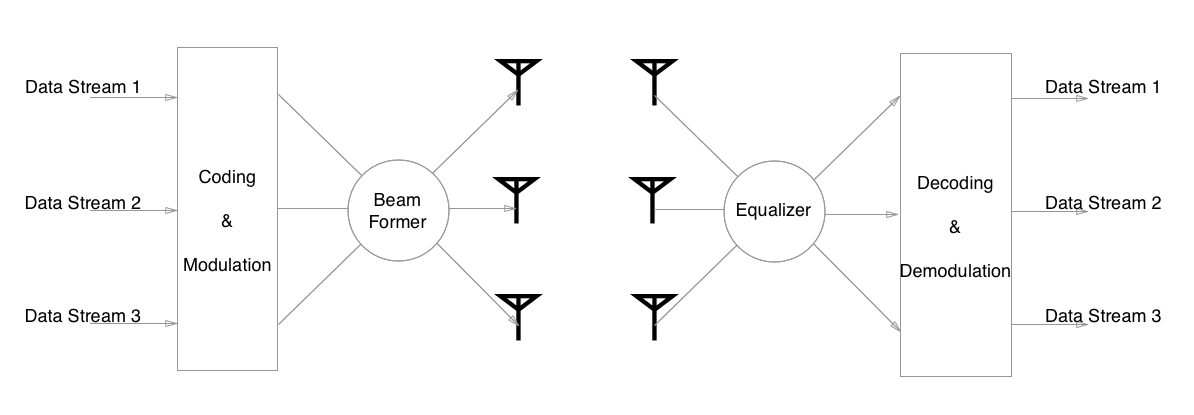
\includegraphics[scale=0.33]{Scenario.png}
\caption{The Scenario Model}
\label{fig:Scenario}
\end{figure}

\noindent
The system is built based on the Orthogonal Frequency Division Multiplexing and a binary data stream of a resource block length is transmitted for each user at each time slot.
The data streams would be coded and modulated into the signal sequences.
The sequences would be processed by the beam former to eliminate the inter-user interference.
The processed sequence would be transmitted through the channel and the received signal of a user \textit{k} is modelled as:
\subsection{Channel Model}
The channel bewteen the $\textit{i}$th transmission antenna and the $\textit{k}$th user is modelled as a complex gain:
\[H_{ki} = a+bj\]
Therefore the channels between the base station and the users are modelled as a matrix of size $\textit{K}*\textit{I}$:
\[
\textbf{H}
=
\begin{bmatrix}
    \textbf{H}_{11} & \textbf{H}_{12} & \textbf{H}_{13} & \dots  & \textbf{H}_{1I} \\
    \textbf{H}_{21} & \textbf{H}_{22} & \textbf{H}_{23} & \dots  & \textbf{H}_{2I} \\
    \vdots & \vdots & \vdots & \ddots & \vdots \\
    \textbf{H}_{K1} & \textbf{H}_{K2} & \textbf{H}_{K3} & \dots  & \textbf{H}_{KI}
\end{bmatrix}
\]
The channel for user $\textit{k}$ is thus a row vector:
\[
\textbf{H}_k
=
\begin{bmatrix}
    \textbf{H}_{k1} & \textbf{H}_{k2} & \textbf{H}_{k3} & \dots  & \textbf{H}_{kI}
\end{bmatrix} \hspace{1cm}(k = 1,...,K)
\]
The received signal for the \textit{k}th user could be derived as:
\[
\textbf{y}_k = \textbf{H}_k\textbf{x}+\textbf{n}_k = \textbf{H}_{k1}\textbf{x} + \textbf{H}_{k2}\textbf{x} +
\dots + \textbf{H}_{kI}\textbf{x} + \textbf{n}_k \hspace{1cm}(k = 1,...,K)
\]
Where \textbf{x} is the beamformed sequence from the base station antennas, $\textbf{H}_k$ is the channel matrix for the $\textit{k}$th user,
$\textbf{n}_k$ is the additive white Gaussian noise (AWGN) for the $\textit{k}$th user, and $\textbf{y}_k$ to be the received signal for the $\textit{k}$th user.

\subsection{Zero-Forcing Beam Former}
The beam former is designed to eliminate the inter-user interference. It could be modelled as a matrix of size $\textit{I}*\textit{K}$
\[
\textbf{W}
=
\begin{bmatrix}
    \textbf{W}_{11} & \textbf{W}_{12} & \textbf{W}_{13} & \dots  & \textbf{W}_{1K} \\
    \textbf{W}_{21} & \textbf{W}_{22} & \textbf{W}_{23} & \dots  & \textbf{W}_{2K} \\
    \vdots & \vdots & \vdots & \ddots & \vdots \\
    \textbf{W}_{I1} & \textbf{W}_{I2} & \textbf{W}_{I3} & \dots  & \textbf{W}_{IK}
\end{bmatrix}
\]
The beamformer for each user becomes the colomn vector:
\[
\textbf{W}_k
=
\begin{bmatrix}
    \textbf{W}_{1k} \\
    \textbf{W}_{2k} \\
    \vdots \\
    \textbf{W}_{Ik}
\end{bmatrix} \hspace{1cm}(k = 1,...,K)
\]
The processed signal sequence would thus be:
\[
\textbf{x} = \textbf{WS} = \textbf{W}_1\textbf{s}_1 + \textbf{W}_2\textbf{s}_2 + \dots +\textbf{W}_K\textbf{s}_K
\]
And the received signal for \textit{k}th user would be:
\[
\textbf{y}_k = \underbrace{\textbf{H}_k\textbf{W}_1\textbf{s}_1 +\textbf{H}_k\textbf{W}_2\textbf{s}_2+\textbf{H}_k\textbf{W}_3\textbf{s}_3
+\dots}_{interference}+\overbrace{\textbf{H}_k\textbf{W}_k\textbf{s}_k}^{signal}+
\underbrace{\dots+\textbf{H}_k\textbf{W}_K\textbf{s}_K}_{interference} +\underbrace{\textbf{n}_k}_{noise}
\]
\[
\textit{k} = 1,2,\dots,\textit{K}
\]
The zero-forcing beamformer is designed to eliminate the inter-user interference completely,i.e.,to make the interference part in the received signal equal to 0.
\[
\textit{interference} = \sum_{k' = 1,k'\neq k}^{k' = K}\textbf{H}_k\textbf{W}_{k'}\textbf{s}_{k'} = 0
\]
As $\textbf{s}_{k'}$ is the signal sequence of user \textit{k'}, $\textbf{s}_{k'} \neq 0$, the following condition needs to be fulfilled to cancel out the interference:
\[
\textbf{H}_k\textbf{W}_{k'} = 0 \hspace{1cm}(k \neq k')
\]
From the pespective of the whole system serving \textit{K} users, the beamformer matrix should be designed to match the condition:
\[
\textbf{WH} = \textbf{I}
\]
where I is the identity matrix.

\noindent
Solving this condition, the zero-forcing beamformer \textbf{W} would be the pseudo-inverse of the channel matrix \textbf{H}:
\[
\textbf{W} = \textbf{H}^{\dagger} = \textbf{H}^H(\textbf{H}\textbf{H}^H)^{-1}
\]
\subsection{Power Allocation}
The original beamformer would have a power gain larger than 1 which make the signal power exceeding the maximum output of the transmission antennas.
In this situation, the beamformer has to be rescaled to fulfill the power constraint.
Two different rescale methods are applied to meet the power limitation while allocate different power to different users.
The power constraint for each transmission antenna is set to be 1 for simplicity.

\subsubsection{Equal Power Scaling Allocation Scheme}
In the normalized scheme, the beam former matrix is normalized by its Frobenius Norm:
$$
\textbf{W} = \frac{\textbf{W}}{norm(\textbf{W}, 'fro')}
$$
This normalization process would simply rescaled the whole matrix with a constant to fulfill the limitation.
Power is equally allocated for each user.
\subsubsection{Water Filling Scheme}
The water filling scheme is targeted to reach a maximum data rate for the whole group of users.
The method would allocate more power to those with better channel state to boost their achievable rate while meeting the power constraint.
$$
\max \sum_{n=1}^{N_U} log(1+p_n)
$$
with the limitation of
$$\sum_{n=1}^{N_U} p_n \leq 1$$
Iterative division method is applied to find the value of $p$ to maximize the achievable rate.

\subsection{Simulation Platform}
The system diagram for the simulation platform is shown in figure 2.
\begin{figure}[ht]
\centering
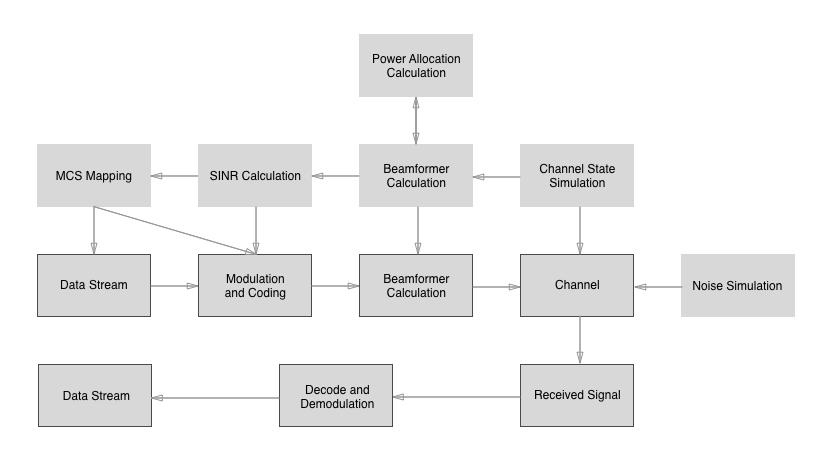
\includegraphics[scale=0.5]{SystemDia.png}
\caption{The System Diagram}
\label{fig:SystemDia}
\end{figure}

\noindent
The channel matrix \textbf{H} is firstly generated randomly and the corresponding beamformer \textbf{W} is calculated.
Additive white Gaussian noise is generated as a random vector $\textbf{n}_k$ for the \textit{k}th user with the noise power $\sigma^2$.
A data stream of a block length is simulated for each user for transmission.
Signal-to-Interference-and-Noise-Ratio for each user is then calculated to determine the modulation and coding scheme.
The SINR for the \textit{k}th user is:
\[
SINR_k = \frac{Signal}{Interference+Noise} = \frac{\textbf{H}_k\textbf{W}_kP_{sk}}{\sum_{k' = 1,k'\neq k}^{k' = K}\textbf{H}_k\textbf{W}_{k'}\textbf{s}_{k'}P_{sk'}+\sigma^2}
\]
where $P_{sk}$ is the power of signal $\textbf{s}_k$ and $P_{sk'}$ is the power of signal $\textbf{s}_k'$.

\noindent
The SINR is converted into decimal scale and mapped to the corresponding CQI and MCS index values.
$$SINR(dB)_k = 10*log_{10}(SINR)$$
With the specific modulation and coding scheme, the data stream is converted into the signal sequence and simulation transmission is performed.

\noindent
The decoded data stream at the user side would be compared to the original one for evaluation.


\section{Performance Evaluation}
The detected data streams are compared to the original ones and check if there is any error. The blocks successfully transmitted are counted to the total throughput.
\[ThroughPut_k = L_{Bl}N_{Bl}\]
where $L_{Bl}$ is the block length of the specific modulation and coding scheme and the $N_{Bl}$ is the number of blocks which are transmitted correctly.

\noindent
The achievable rate for the \textit{k}th user is calculated from the SINR values:
$$AcRate_k = F*Bandwidth*log_2(1+SINR)$$
\begin{center}(F : system loss of the OFDM)\end{center}
The comparison between the total throughput and the total achievable rate for all users is conducted to evaluate the performance.
The performance of the system applying the two power allocation schemes is shown in figure 3 (2-user-2-input-single-output system).


\begin{figure}[ht]
\centering
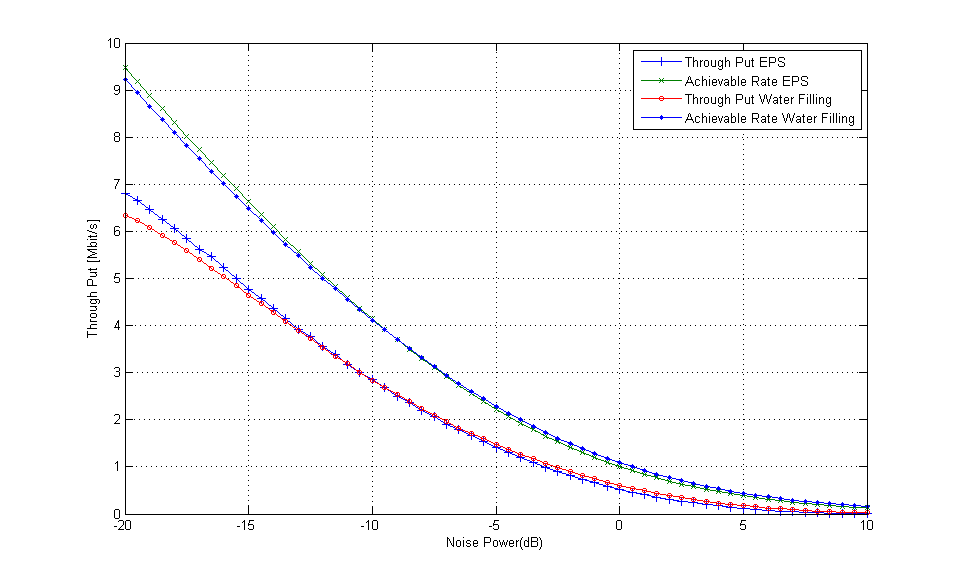
\includegraphics[scale=0.45]{WFvsEPS.png}
\caption{Water Filling vs EPS Comparison}
\label{fig:MUSOvsSISO}
\end{figure}

\noindent
The waterfilling power allocation method performs better in the total through put with high noise power.
The EPS method outperforms the waterfilling method when the noise power is low. This should be caused by the limitation of maximum transmit rate of the modulation and coding schemes.

\noindent
The performance of the adaptive Single-Input-Single-Output(SISO) system is shown in figure 4. Comparing figure 3 and figure 4,
 performance is much boosted for the zero-forcing MU-MISO system comparing to the SISO system with both power allocation schemes.
\begin{figure}[ht]
\centering
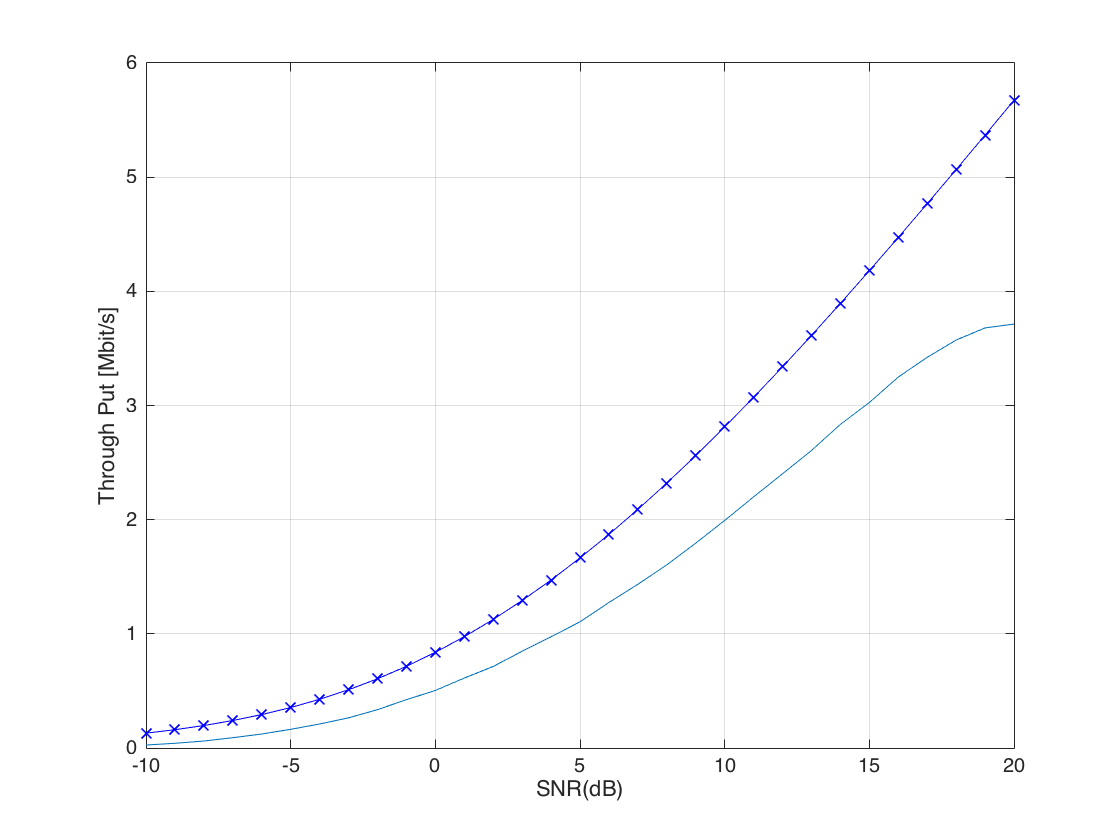
\includegraphics[scale=0.25]{FadingSISO.png}
\caption{SISO Performance}
\label{fig:WFvsEPS}
\end{figure}


\section{Conclusion}
The multi-antenna communication system have a much better net through put performance than the single antenna system.
The multi-antenna technology would be replacing the SISO system in modern communication systems to achieve better performances for
real-world multi-user scenarios.

\noindent
The water filling algorithm outperforms the EPS scheme in term of total throughput at high noise power but loses the advantage at low noise power.
The failing of the water filling algorithm when the channel quality is good should be further researched and the algorithm should be
improved to overcome the problem.
\end{document}
